% Created 2021-11-26 Fri 16:03
% Intended LaTeX compiler: pdflatex
\documentclass[11pt]{article}
\usepackage[utf8]{inputenc}
\usepackage[T1]{fontenc}
\usepackage{graphicx}
\usepackage{grffile}
\usepackage{longtable}
\usepackage{wrapfig}
\usepackage{rotating}
\usepackage[normalem]{ulem}
\usepackage{amsmath}
\usepackage{textcomp}
\usepackage{amssymb}
\usepackage{capt-of}
\usepackage{hyperref}
\author{Rodrigo Castillo Camargo, Alejadra Campo Archbold, Juan Pablo Sierra Useche}
\date{\today}
\title{¿Cómo suena Colombia?}
\hypersetup{
 pdfauthor={Rodrigo Castillo Camargo, Alejadra Campo Archbold, Juan Pablo Sierra Useche},
 pdftitle={¿Cómo suena Colombia?},
 pdfkeywords={},
 pdfsubject={},
 pdfcreator={Emacs 27.1 (Org mode 9.5)}, 
 pdflang={English}}
\begin{document}

\maketitle

\section{Resumen}
\label{sec:org3eda03d}
Colombia es un país muy diverso, debido a las diferentes culturas y movimientos
culturales que hay en nuestro país el panorama de la música es bastante difuso,
esto porque para los músicos resulta una tarea titánica tratar de entender los
sonidos y las corrientes musicales que hay en nuestro país e identificar
patrones sobre ellos ya que para lograr esto se tendría escuchar la música de
todas las agrupaciones en Colombia. Además, es una tarea muy difícil intentar
llevar un registro formal de las agrupaciones musicales en el país puesto que
las bandas musicales no siempre están registradas en las mismas plataformas,
además, constantemente están naciendo nuevas bandas musicales y a su vez van
muriendo otras.

El análisis estadístico de datos es una rama de las ciencias de la computación
que permite inferir distintas propiedades de los datos a partir de métodos que
se sustentan en la estadística, generalmente, responde a tres problemas
específicos; la predicción  de factores , la clasificación y el agrupamiento.
Éstas herramientas fueron de gran ayuda para ampliar nuestros conocimientos
sobre los sonidos musicales que hay en Colombia.

En este informe se hizo un análisis de la música en colombia usando métodos del
análisis estadístico de datos, de esta forma, se pueden inferir patrones en la
música colombiana que pueden facilitar una aproximación a la exploración del
panorama de la música en Colombia.

\section{Preguntas}
\label{sec:org3cfbf60}
Una de las principales motivaciones que tuvo este informe era entender que tipos
de agrupaciones musicales hay en Colombia y visualizarlas, ya que siendo un país
tan diverso, desde la perspectiva del análisis de datos , ¿cuáles tipos de
música predominan en el país? , ¿cuántas y cuales agrupaciones de grupos que
cumplen los mismos patrones existen?.

Otra de las motivaciones que tuvo este informe fue entender desde un fin
comercial de la música que factores pueden influir en la popularidad de una
banda y proponer una estrategia para las bandas musicales que pueda aumentar su
popularidad en plataformas como Spotify. Además, ver si es posible predecir la
popularidad de una canción según factores que estén implícitos en su respectivo
mel-espectrograma.

\section{Métodos Usados}
\label{sec:org3bd977e}
\subsection{Respecto a la recolección de datos:}
\label{sec:orgfe31b41}
Puesto que no existe una base de datos que contenga información sobre las bandas
en Colombia y sus diferentes sonidos, el grupo optó por generar su propia tabla
de datos utilizando técnicas de recolección de datos  de revistas de música en
Colombia, para esto se usaron librerias de python tales como Selenium, bs4 y
requests.

Se recolectaron los nombres de las bandas que están en el bomm (Bogotá Music
Market) , en Circulart , en La FM y además se añadieron las bandas que están
registradas en el SIMUS. Posteriormente, a cada banda se le hizo una búsqueda en
spotify para relacionarla con variables que la API de spotify proporciona, tales
como la bailabilidad de ésta, la media del tempo de sus canciones, la
popularidad, la duración promedio de sus canciones\ldots{}etc.

\subsection{Respecto a la descripción de el sonido específico de una canción y la reducción de dimensionalidad:}
\label{sec:org49b4adf}
Una vez teniendo los nombres de las bandas , se descargó la canción mas popular
de cada banda de youtube y se calculó su respectivo mel-espectrograma , sin
embargo, esto suponía un problema de memoria, puesto que no es posible almacenar
miles de espectrogramas de canciones en la RAM de los computadores de los
integrantes del grupo. La solución a este problema es que, al ser los
mel-espectrogramas matrices de la forma \(A=128\times k\) en donde \(k\) representa
el sampleo con respecto al tiempo de una canción , fue posible aplicar métodos
de reducción de dimensionalidad como PCA(Principal Component Analysis) para
representar el sonido de las canciones en vectores de 128 dimensiones, en los
que cada variable representa valores singulares del resultado de reducir la
dimensionalidad del mel-espectrograma.

Adicionalmente, como uno de los propósitos del proyecto era visualizar los
distintos sonidos que hay en nuestro país, se adicionaron dos variables extras
que son el resultado de reducir la dimensionalidad de cada mel-espectrograma a 2
dimensiones, esto con el fin de poder graficar los sonidos de cada banda musical
en 2 dimensiones.

El grupo es consciente de que una canción no es suficiente para representar el
sonido de una banda, por lo que se planteó la opción de concatenar varias
canciones, sin embargo, aunque está implementado, el grupo se vió forzado a
optar por la canción más popular de cada agrupación debido a que el proceso de
reducir la dimensionalidad de la concatenación de varias canciones es pesado
computacionalmente y había limitaciones de hardware. El proceso de reducir la
dimensionalidad de una canción por banda tomó al rededor de 10 días en una
máquina T2-micro de AWS.

\subsection{Respecto a la agrupación(clustering):}
\label{sec:org434dd14}
Como uno de los propósitos del proyecto era entender que tipos de agrupaciones
musicales hay en nuestro país, se implementó K-Means sobre los vectores que
representaban el sonido de cada banda

\subsection{Respecto al Análisis de Correlaciones:}
\label{sec:orgf9b7915}
Se implementó un modelo de regresión lineal para detectar si había correlaciones entre los sonidos de las canciones y la popularidad de las bandas

\subsection{Respecto a la predicción de la popularidad de canción:}
\label{sec:orgc22857b}
Se implementó un modelo de una regresión logística para intentar diferenciar
bandas populares de bandas impopulares, sin embargo, esto no funcionó, por lo
que, el grupo siendo consciente de que el tema no fue parte del curso de
análisis de datos, se implementó un modelo de random forest que obtuvo mucho
mejores resultados.

\section{Resultados:}
\label{sec:org6c54510}
\subsection{Respecto a la agrupación(clustering):}
\label{sec:org291aa62}
la siguiente gráfica muestra la inercia que conserva la cantidad de clusters
establecidos por los vectores representantes del sonido de cada banda.

\begin{center}
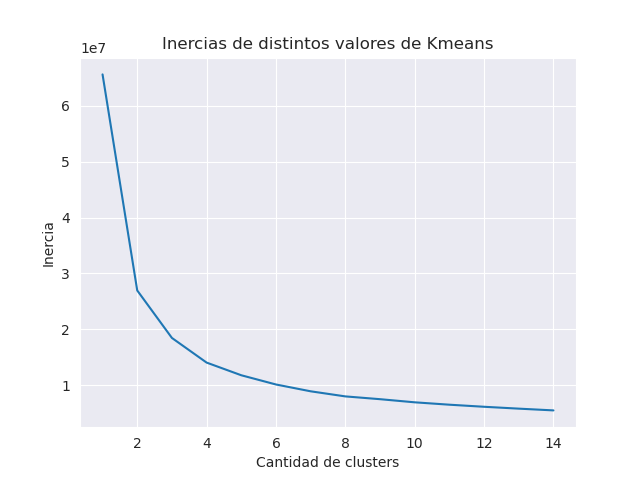
\includegraphics[width=.9\linewidth]{./images/inercias1.png}
\end{center}

Usando el criterio del codo, se estableció
que 3 sería un buen número de clusters para estos datos, así, luego de
implementar K-Means y analizar el contenido de cada grupo, se obtuvieron los
siguientes resultados:

\begin{center}
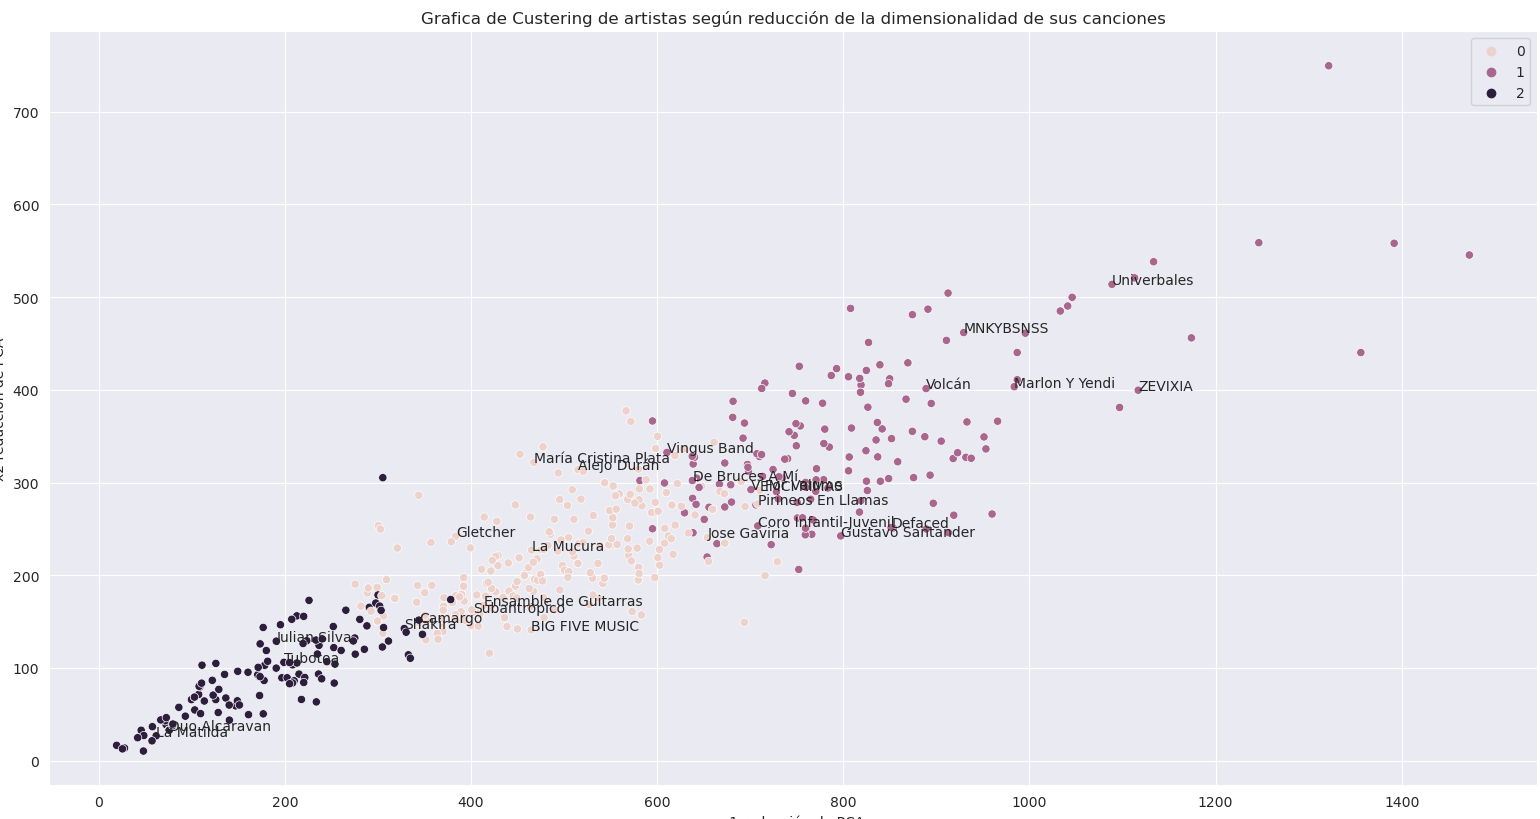
\includegraphics[width=.9\linewidth]{./images/clustering1.png}
\end{center}

\subsubsection{Discusión}
\label{sec:orgbfe8ecc}
En estos clusters se pueden apreciar las siguientes regularidades:
\begin{enumerate}
\item el grupo de más a la izquierda(2-negro) contiene bandas pertenecientes a la escena indie-alternativa en Colombia
\item el grupo del medio (0-ocre) contiene bandas pertenecientes a la escena pop en Colombia
\item el grupo de la derecha(1-morado) contiene bandas que frecuentan sonidos latinoamericanos (reggaeton, dancehall , música del pacífico\ldots{}etc)
\end{enumerate}

de los siguientes grupos se puede ver que las variables que mas los diferencian
son:
\begin{enumerate}
\item la popularidad.
\item la varianza de la popularidad.
\item las varianzas de tempo en las canciones de los artistas.
\end{enumerate}

\begin{center}
\begin{tabular}{lrrrr}
 & Cluster 0 & Cluster 1 & Cluster 2 & Varianza\\
\hline
popularity mean & 9.63778 & 6.57615 & 7.56232 & 1.62818\\
popularity variance & 69.5904 & 54.5974 & 56.1064 & 45.4319\\
duration mean & 226307 & 234865 & 235132 & 1.67981e+07\\
duration variance & 3.896e+09 & 4.71516e+09 & 4.31885e+09 & 1.11878e+17\\
tempo variance & 807.326 & 780.103 & 781.798 & 155.064\\
\end{tabular}
\end{center}

De esto se puede concluir que:

\begin{enumerate}
\item Aunque las bandas que pertenecen al grupo de la derecha(1-morado) tienden a ser mas populares que las de los otros grupos, también hay más varianza de popularidad, es decir que, hay artistas sumamente populares pero también hay artistas muy desconocidos que frecuentan estos ritmos
\item Las popularidades de las bandas que no pertenecen al grupo de sonidos latinoamericanos es muy parecida, sin embargo, la varianza de popularidad del grupo de pop es menor a la de los otros grupos, por lo que, para una empresa discográfica, invertir dinero en una banda de pop representa un riezgo menor que invertirlo en una banda de indie
\item La varianza de tempo en el grupo de la música latinoamericana es mayor que en los otros dos grupos, esto se debe a que en este género hay artistas que tienen canciones muy diferentes entre si.
\item el resto de variables de spotify no proporciona información que sea considerada por la agrupación de K-Means
\item Aún cuando históricamente la humanidad haya agrupado a la música en géneros musicales, estos son solamente cateogrías que se han asignado por fines comerciales, sin embargo pueden existir otras formas de agrupar la música según otros criterios u otras métricas, los distintos algoritmos de aprendizaje no supervisado pueden proporcionar diferentes visiónes del panorama musical que no necesariamente estén ligadas a géneros musicales.
\end{enumerate}

\subsection{Respecto al análisis canónico de Correlaciones}
\label{sec:org78d3d90}
Se intentó ver si había una correlación lineal entre el sonido de las bandas y su popularidad, para esto se implementó un modelo simple de regresión lineal y se obtuvieron los siguientes resultados:
\begin{center}
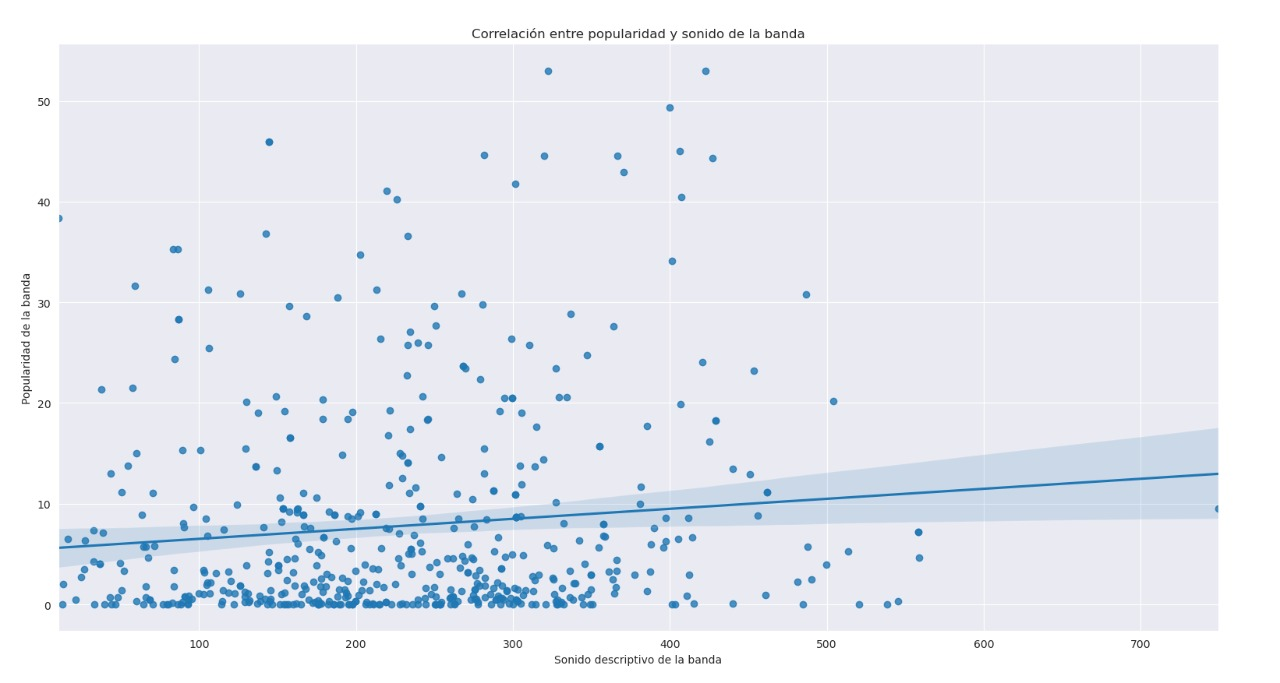
\includegraphics[width=.9\linewidth]{./images/corr1.jpeg}
\end{center}
\subsubsection{Discusión:}
\label{sec:org3f42d4b}
\begin{enumerate}
\item Se puede notar que existe una correlación lineal muy leve entre el sonido de las bandas y su popularidad en spotify, sin embargo, esta correlación no es muy fuerte.
\item El hecho de que no existan correlaciones lineales entre ambas variables no quiere decir que no estén correlacionadas de otras formas, esto puede ser un caso de estudio para el proyecto.
\end{enumerate}


\subsection{Respecto a la clasificación según la popularidad}
\label{sec:org17912d3}

De los vectores descriptivos del sonido de cada banda se intentó hacer un modelo
que fuera capáz de predecir si una banda iba a ser popular o no según la
plataforma de spotify desde la forma en la que suena. Inicialmente se intentó
hacer un modelo de regresión logistica simple, sin embargo, este no tuvo buenos
resultados puesto que los vectores de sonido de las canciones no guardan una
relación muy lineal con la popularidad de las bandas de spotify. Finalmente, se
entrenó un modelo de Random Forest sobre los mismos datos que tuvo mejores
resultados que el modelo de regresión logística:


\begin{center}
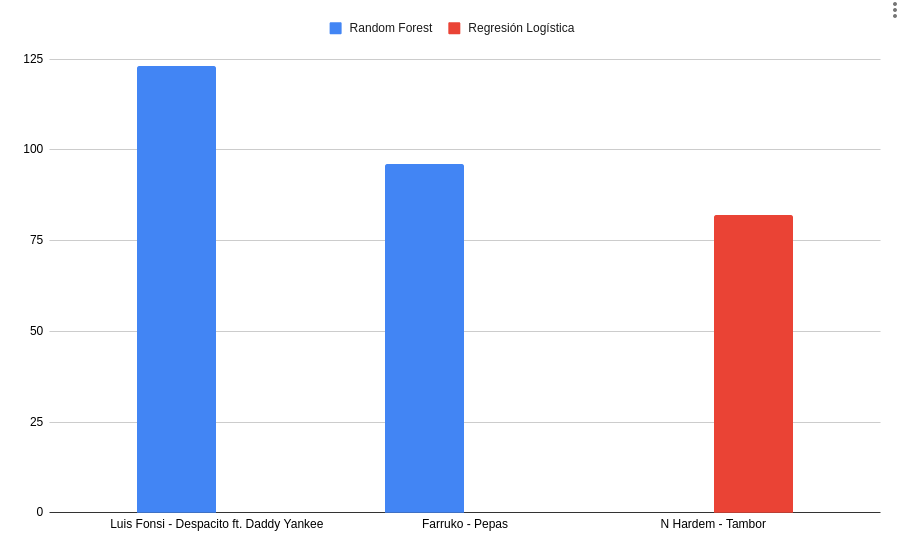
\includegraphics[width=.9\linewidth]{images/hist1.png}
\end{center}

\begin{center}
\begin{tabular}{lr}
Canción & Regresión Logística\\
\hline
Los Saicos - Demolición & 34\\
Hit The Button Karaoke - Lo Siento Bb & 304\\
Rels B - A Mí & 290\\
Conociendo Rusia - No Aguanto Más & 0\\
Sidestepper - Mas Papaya & 0\\
FrioLento - Bichota (Post-Punk) & 24\\
Bad Bunny - Si Veo a Tu Mamá & 0\\
Esteman, Daniela Spalla - Te Alejas Más De Mí & 0\\
Duplat, Santiago Navas - Lo Que Pudimos Ser & 186\\
C. Tangana, ROSALÍA - Antes de Morirme & 354\\
\end{tabular}
\end{center}

\begin{center}
\begin{tabular}{lr}
Canción & Random Forest\\
\hline
Los Saicos - Demolición & 315\\
Hit The Button Karaoke - Lo Siento Bb & 59\\
Rels B - A Mí & 290\\
Conociendo Rusia - No Aguanto Más & 0\\
Sidestepper - Mas Papaya & 225\\
FrioLento - Bichota (Post-Punk) & 0\\
Bad Bunny - Si Veo a Tu Mamá & 0\\
Esteman, Daniela Spalla - Te Alejas Más De Mí & 0\\
Duplat, Santiago Navas - Lo Que Pudimos Ser & 0\\
C. Tangana, ROSALÍA - Antes de Morirme & 107\\
\end{tabular}
\end{center}

\subsubsection{Discusión:}
\label{sec:orge00ed05}
\begin{enumerate}
\item Los vectores que describen el sonido de cada canción tienen comportamientos muy poco lineales, por lo que una regresión logística no puede relacionar esta clase de valores con la popularidad de una canción, sin embargo, modelos como Random Forest si pueden, haciendo posibles herramientas para la predicción de la popularidad de bandas en plataformas como spotify.
\item Como se puede ver, en ambos modelos hay situaciones en las que los resultados no tienen sentido, esto porque los modelos fueron entrenados con datos de bandas en Colombia, también, porque la popularidad de una canción no solamente depende del sonido de una banda o un artista, sino de la fama de éste. Esto puede dar paso a un trabajo futuro en el que se estudie esta clase de comportamientos teniendo en cuenta la popularidad previa de los artistas.
\end{enumerate}




\section{Bibliografía:}
\label{sec:org03d1741}
\subsection{Bomm:}
\label{sec:orgd5b2342}
El BOmm(Bogotá Music Market) es una revista en la cuál se registran bandas que
frecuentan en Bogotá: referencia : \url{https://www.bogotamusicmarket.com/}
\subsection{Circulart:}
\label{sec:orgcb44059}
Circulart es una revista en la cuál se registran bandas que frecuentan en
Medellín referencia :  \url{https://circulart.org/2021/}
\subsection{SIMUS:}
\label{sec:org09787ec}
El SIMUS es una base de datos en la cuál se tienen que registrar todas las
bandas que tienen contratos con el estado referencia :
\url{https://simus.mincultura.gov.co/}
\subsection{LastFM:}
\label{sec:org841e416}
LastFM es una página que contiene mucha información sobre artistas, contiene la
categoría de artistas colombianos por lo que fue de grán ayuda para este
proyecto referencia : \url{https://www.last.fm}

\section{Anexos:}
\label{sec:org7b1b368}

Todo el proyecto fue desarrollado en el siguiente repositorio:
\url{https://github.com/Rootdrigo/Colombian\_Music\_State}
\end{document}
